% Copyright 2023 The terCAD team. All rights reserved.
% Use of this content is governed by a CC BY-NC-ND 4.0 license that can be found in the LICENSE file.

\subsection{Benchmarking Prototype}
\markboth{Unleashing Features}{Benchmarking Prototype}

Before adding functionality in the form of muscles to the created prototype skeleton, we need to verify its reliability.
Restructuring the fundamental concepts of the application in the future would not only pose a considerable challenge 
but also entail a substantial effort and potential complications.


\subsubsection{Providing Integration Tests}

Unit (\ref{ut-unit}) and widget (\ref{widget-tests}) tests serve as valuable tools for assessing isolated classes, 
functions, or widgets. However, not all of the problems can be tackled by them. Integration tests are used to identify 
systemic flaws (data corruption, concurrency problems, miscommunication between services, etc.) that might not be 
evident in unit tests by verifying a synergy of individual assets, validating the application as a whole. 
Integration tests are designed to reflect the real-time performance of an application on an actual device or platform. 
In conclusion, they provide a vital link in the testing hierarchy by validating a collocation of various components 
within an application. In such a way integration tests simulate end-to-end user workflows that we've implemented and 
discussed earlier -- \ref{t-gherkin}.

Integration tests in Flutter can be written by using \q{integration\_test}-package, \q{flutter\_driver}-package would 
help us to evaluate our tests on real / virtual devices and environments and track the timeline of tests execution 
(both packages are provided by the SDK):

\begin{lstlisting}[language=yaml]
## ./pubspec.yaml
dev_dependencies:
  integration_test:
    sdk: flutter
  flutter_driver: 
    sdk: flutter
\end{lstlisting}

\noindent The implementation's deference from a widget test is in a usage of the next code line, that enables tests 
execution on a physical device or platform:
\begin{lstlisting}
IntegrationTestWidgetsFlutterBinding.ensureInitialized();
\end{lstlisting}

\q{Firebase Test Lab} and \q{BrowserStack} stand as a cloud-powered testing platforms, and enable the integration tests
evaluation across an extensive spectrum of devices and configurations.


\subsubsection{Doing Performance Testing}

Performance testing is a type of software testing designed to evaluate the speed, responsiveness, stability, and 
overall performance of an application under different conditions. It involves subjecting the application to 
simulated workloads and stress scenarios to assess how it behaves in terms of speed, scalability, and resource usage. 
Performance testing ensures that the software can handle the expected load without degradation in performance.

By simulating different levels of user traffic, performance testing helps determine the application's scalability by
assessing resources utilization (CPU, memory, network bandwidth, and other parameters), and identify performance 
bottlenecks, such as slow database queries, inefficient code, or network latency, and address these issues before 
they will impact users.

The detailed information about performance testing can be taken from the International Software Testing Qualifications 
Board (ISTQB) or the Software Engineering Institute (SEI), while here we'll highlight only their types definition 
(\cite{Ian15}, \cite{Sag16}, \cite{Sag23}):
\begin{itemize}
  \item Load Testing: Evaluates how an application performs under expected load conditions. It helps determine the 
  application's response time, resource utilization, and overall stability.

  \item Stress Testing: Pushes the application to its limits by subjecting it to extreme conditions, such as excessive 
  user loads or resource scarcity. It aims to identify the breaking point and understand how the application recovers 
  from failures.

  \item Endurance Testing: Assesses the application's performance over an extended period to identify issues related to 
  memory leaks, resource exhaustion, or gradual degradation in performance.

  \item Spike Testing: Simulates sudden spikes in user traffic to assess how the application responds to rapid changes
  in load. This helps uncover bottlenecks and issues related to sudden surges in demand.

  \item Volume Testing: Focuses on testing the application's performance with large volumes of data, such as a high 
  number of records in a database. It helps identify scalability and performance issues associated with data volume.
\end{itemize}

\noindent Back to our process, it would be used the next command to evaluate performance tests:

\begin{lstlisting}[language=bash]
# Precondition for Web profiling
chromedriver --port=4444
# Launch tests
flutter drive \
  --driver=test_driver/perf_driver.dart \
  --target=integration_test/name_of_test.dart \
  --profile
\end{lstlisting}

The \q{--profile}-option enables the application compilation in "profile mode" that helps the benchmark results to be
closer to what will be experienced by end users. By running on a mobile device or emulator it's proposed to use 
\q{--no-dds}-parameter in addition, that will disable unaccessible Dart Development Service (DDS). The \q{--target} 
declares the scope of test executions while \q{--driver}-option does track the outcomes. The driver configuration can be
taken from \href{https://docs.flutter.dev/cookbook/testing/integration/profiling}{https://docs.flutter.dev/cookbook/testing/integration/profiling}:

\begin{lstlisting}
// ./test_driver/perf_driver.dart
import 'package:flutter_driver/flutter_driver.dart' as driver;
import 'package:integration_test/integration_test_driver.dart';

Future<void> main() {
  return integrationDriver(
    responseDataCallback: (data) async {
      if (data != null) {
        final timeline = driver.Timeline.fromJson(data['timeline']);
        final summary = driver.TimelineSummary.summarize(timeline);
        await summary.writeTimelineToFile(
          'timeline',
          pretty: true,
          includeSummary: true,
          destinationDirectory: './coverage/',
        );
      }
    },
  );
}
\end{lstlisting}

\noindent Since it's a Widget Tests'-based approach (\ref{widget-tests}, \ref{t-gherkin}), we'll accent only on the 
usage of \q{traceAction}-method to store time-based metrics:

\begin{lstlisting}
// ./test/performance/load/creation_test.dart
void main() {
  final binding = IntegrationTestWidgetsFlutterBinding.ensureInitialized();
  testWidgets('Cover Starting Page', (WidgetTester tester) async {
    await binding.traceAction(() async {
        // ... other steps
        final amountField = find.byWidgetPredicate((widget) {
          return widget is TextField && widget.decoration?.hintText == 'Set Balance';
        });
        await tester.ensureVisible(amountField);
        await tester.tap(amountField);
        // In profiling mode some delay is needed:
        await tester.pumpAndSettle(const Duration(seconds: 1));
        // await tester.pump();
        await tester.enterText(amountField, '1000');
        await tester.pumpAndSettle();
        expect(find.text('1000'), findsOneWidget);
        // ... other steps
      },
      reportKey: 'timeline',
    );
  });
}
\end{lstlisting}

\noindent Generated \q{timeline.timeline.json}-file can be traced by \q{chrome://tracing/} in Google Chrome browser 
(\cref{img:perf-chrome-tracing}):

\img{features/perf-chrome-tracing}{Google Chrome -- performance trace}{img:perf-chrome-tracing}

\noindent The \q{timeline.timeline\_summary.json}-file, by being a native \q{JSON}-file, can be opened in IDE for a 
manual check, but it's mostly used in CI/CD to fail the build if any of defined parameter is out of the declared range. 

By example, the value of \q{average\_frame\_build\_time\_millis}-parameter is recommended to be below 16 milliseconds to 
ensure that the app runs at 60 frames per second without glitches. Other parameters are widely described on the page --
\href{https://api.flutter.dev/flutter/flutter\_driver/TimelineSummary/summaryJson.html}{https://api.flutter.dev/flutter/flutter\_driver/TimelineSummary}.


\subsubsection{Measuring Responsiveness}
\paragraph{Load Testing}
Check response time and resource utilization for the first run (Initial Setup) by creating account and budget 
category:

\begin{lstlisting}[language=cucumber]
@start
Feature: Verify Initial Flow
  Scenario: Applying basic configuration through the start pages
    Given I am firstly opened the app
    Then I can see "Initial Setup" component
    When I tap "Save to Storage (Go Next)" button
    Then I can see "Acknowledge (Go Next)" component
    When I tap "Acknowledge (Go Next)" button
    Then I can see "Create new Account" component
    When I tap on 0 index of "ListSelector" fields
    And I tap "Bank Account" element
    And I enter "New Account" to "Enter Account Identifier" text field
    And I enter "1000" to "Set Balance" text field
    And I tap "Create new Account" button
    Then I can see "Create new Budget Category" component
    When I enter "New Budget" to "Enter Budget Category Name" text field
    And I enter "1000" to "Set Balance" text field
    When I tap "Create new Budget Category" button
    Then I can see "Accounts, total" component
\end{lstlisting}

\noindent And, what we've identified from executions (\cref{tb:frame-build}) is a degraded \q{frame build}-parameter 
that affects our frames per second (FPS) by generating only 37 frames instead of 60:\\

\begin{table}[h!]
  \begin{tabular}{ |p{6.8cm}||r|r|r|  }
    \hline
    \multicolumn{4}{|c|}{Frame Build Time, in milliseconds} \\
    \hline
    Type of state & Cold Start & Retrial & With Data\\
    \hline
    average          &  26.00 &  24.28 &  29.65 \\
    90th percentile  &  47.20 &  43.38 &  70.33 \\
    99th percentile  & 158.31 & 159.41 & 198.03 \\
    \hline
  \end{tabular}
  \caption{Performance Test Results for Feature "Verify Initial Flow"} \label{tb:frame-build}
\end{table}

\img{features/perf-slow-frame}{Performance Monitor in Visual Studio Code}{img:perf-slow-frame}

\noindent This issue (\cref{img:perf-slow-frame}) pertains to a compilation jank in animations due to shaders 
calculation (a code snippets executed on a graphics processing unit [GPU] to render a sequence of draw commands). 
Their pre-compilation strategy mitigates the compilation-related disruptions during subsequent animations, and improves 
frames per second rendering. To run the app with \q{--cache-sksl} turned on to capture shaders in SkSL:

\begin{lstlisting}[language=bash]
flutter run --profile --cache-sksl --purge-persistent-cache
\end{lstlisting}

\noindent Warm-up shaders in Skia Shader Language (SkSL) format for an application build:

\begin{lstlisting}[language=bash]
# Capture shaders in Skia Shader Language (SkSL) format into a file
flutter drive --profile --cache-sksl --write-sksl-on-exit sksl.json -t test_driver/warm_up.dart
# Build app with SkSL warm-up
flutter build ios --bundle-sksl-path sksl.json
\end{lstlisting}

\begin{lstlisting}
// ./test_driver/warm_up.dart
import 'package:integration_test/integration_test_driver.dart';
Future<void> main() {
  return integrationDriver();(*@ \stopnumber @*)
}

// ./test_driver/warm_up_test.dart
Future<void> main() async {
  IntegrationTestWidgetsFlutterBinding.ensureInitialized();
  SharedPreferencesMixin.pref = await SharedPreferences.getInstance();

  testWidgets('Warm-up', (WidgetTester tester) async {
    await tester.pumpWidget(MultiProvider(
      providers: [
        ChangeNotifierProvider<AppData>(
          create: (_) => AppData(),
        ),
        ChangeNotifierProvider<AppTheme>(
          create: (_) => AppTheme(ThemeMode.system),
        ),
      ],
      child: const MyApp(),
    ));
    await tester.pumpAndSettle(const Duration(seconds: 3));
  });
}
\end{lstlisting}

\noindent Finally, we've taken \q{56 FPS (average)} as an outcome from that tunning.

\subsubsection{Anticipating Churn Rate}
\paragraph{Volume Testing}
Check initial load (a time before the enabled interaction) with a huge transaction log history (32Mb, 128Mb, 
512Mb, 2Gb).

In the context of the current test, our primary objective is to ascertain the time required for the main page to 
become accessible. To achieve this goal, we will monitor the disappearance of the "Project Initialization" header. 
Subsequently, we will contrast this elapsed time with a size of the transactions' log history.

\begin{lstlisting}
// ./integration_test/stress/initialization_test.dart
testWidgets('Cover Initial Page', (WidgetTester tester) async {
  // Start app by using 'pumpWidget'
  await _init(tester);
  FileRunner.tester = tester;
  // Trigger step to verify that data is loaded
  await FirstRun().executeStep();
  // Change test execution timeout (*@ \stopnumber @*)
}, timeout: const Timeout(Duration(minutes: 30)));

// ./test/e2e/_steps/given/first_run.dart
class FirstRun extends Given with SharedPreferencesMixin {
  @override
  RegExp get pattern => RegExp(r"I am firstly opened the app");

  @override
  Future<void> executeStep() async {
    Finder init;
    do {
      init = find.text('Project Initialization');
      await FileRunner.tester.pumpAndSettle(const Duration(microseconds: 50));
    } while (init.evaluate().isNotEmpty);
    await FileRunner.tester.pumpAndSettle();
  }
}
\end{lstlisting}

\begin{figure}
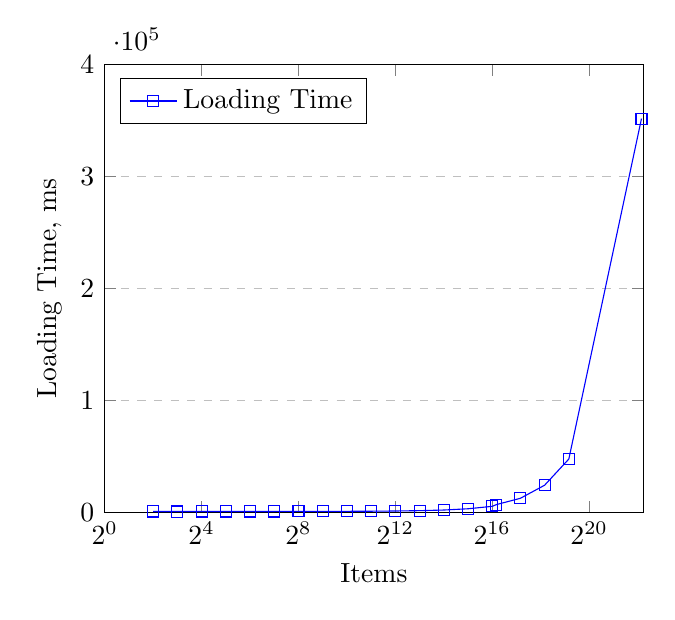
\begin{tikzpicture}
  \begin{axis}[
    xlabel={Items},
    ylabel={Loading Time, ms},
    xmin=0, xmax=5000000,
    ymin=0, ymax=400000,
    xmode=log,
    log basis x={2},
    legend pos=north west,
    ymajorgrids=true,
    grid style=dashed,
  ] 
  \addplot[
    color=blue,
    mark=square,
    ]
    coordinates {
      (0, 863) (4, 935) (8, 887) (16, 937) (32, 931) (64, 932) (128, 957) (256, 1014) (512, 1025) (1024, 1069) 
      (2048, 1169) (4096, 1358) (8192, 1664) (16384, 2221) (32768, 3351) (65536, 5515) (73659, 7064) (146444, 12687)
      (292888, 24353) (585776, 47693) (4686208, 351456)
    };
    \legend{Loading Time}
  \end{axis}
\end{tikzpicture}
\caption{Stress Testing: Loading Time vs. Number of Items} \label{t-stress}
\end{figure}

\noindent Results (\cref{t-stress}) have shown that the needed time for the cold start varies from 863 milliseconds  
with zero items up to 5.85 minutes to load 2.53 GB transactions' log file with 4.7 millions of items. That's far away 
from our assertion -- less than 2 seconds (for the current solution, 8.20 MB file size with 16.4 thousands of items).
This implies that somewhere in between of 1.5 to 5 years of a consistent usage, our customers might encounter a 
situation where opening the application takes longer than 2 seconds. Based on retrieved data, we have to optimize  
initialization by implementing warm-up caching strategy (mostly known as hot, warm, and cold caches \cite{Tom17}). 


\paragraph{Endurance Testing}
Check response time and resource utilization by adding different types of data within a different time 
periods (15 minutes, an hour, 4 hours, 8 hours).

In that test we would be interested in debugging memory issues and CPU profiling that can be achieved via DevTools.
DevTools is a suite of performance and debugging tools for Dart and Flutter that can be started from IDE 
(with installed extensions from \ref{first-step}) by pressing \q{[F1]} and typing \q{devtools} there.

Detecting memory leaks involves analyzing the Heap Snapshot within the Memory View. These snapshots 
(\cref{img:memory-snapshot}) provide a means to compare the heap's growth and identify objects that might exhibit an 
unexpected increase in count. While it's true that images and media can contribute substantially to memory consumption, 
they often aren't the root cause of memory leaks. Instead, attention should be directed towards addressing a potential 
incomplete rebound phenomenon (\cref{img:memory-leak}) for Resident Set Size (RSS, program's memory that is currently 
loaded into RAM and is available for immediate use). A notable illustration of a sizeable, short-lived object that 
could inadvertently infiltrate a long-lived area, consequently leading to leaks, is the \q{context}-parameter 
transmitted to Flutter's build method:

\begin{lstlisting}
Widget build(BuildContext context) {
\end{lstlisting}
{
\xpretocmd{\lstlisting}{\vspace{-12pt}}{}{}
\begin{lstlisting}[firstnumber=2, backgroundcolor=\color{backred}]
(*@\kdiff{-}@*)  // [!] Leak prone issue
(*@\kdiff{-}@*)  final handler = () => apply(Theme.of(context));
\end{lstlisting}
\begin{lstlisting}[firstnumber=2, backgroundcolor=\color{backgreen}]
(*@\kdiff{+}@*)  final theme = Theme.of(context);
(*@\kdiff{+}@*)  final handler = () => apply(theme);
\end{lstlisting}
\begin{lstlisting}[firstnumber=4]
   useHandler(handler);
\end{lstlisting}
}

\img{features/memory-snapshot}{DevTools: Heap Snapshot within the Memory View}{img:memory-snapshot}
\img{features/memory-leak}{Incomplete rebound phenomenon for RSS}{img:memory-leak}
\img{features/devtools-connection}{DevTools: Connect to the running instance}{img:devtools-connection}

\noindent To track CPU and Memory Heap we'll run Devtools separately, and connect it (\cref{img:devtools-connection}) 
to the process by a provided URL from an integration tests' output:

\begin{lstlisting}[language=bash]
Building Windows application...           13.1s
V  Built build\windows\runner\Debug\Fingram.exe.
VMServiceFlutterDriver: Connecting to Flutter application at http://127.0.0.1:52135/VDm4NX0QVr4=/
VMServiceFlutterDriver: Isolate found with number: 3513574544292703
VMServiceFlutterDriver: Isolate is paused at start.
\end{lstlisting}

\noindent The test itself will simulate a user behavior by randomly creating bills (90\%), budget categories (10\%),
and accounts (5\%): 

\begin{lstlisting}
testWidgets('Imitate User Activities', (WidgetTester tester) async {
  final startTime = DateTime.now();
  await cleanUp();
  await firstRun(tester);
  Duration duration;
  int idx = 0;
  final random = Random();
  do {
    if (random.nextDouble() <= 0.05) await createAccount(tester, idx);
    await FileRunner.tester.pumpAndSettle(const Duration(seconds: 5));
    if (random.nextDouble() <= 0.10) await createBudget(tester, idx);
    await FileRunner.tester.pumpAndSettle(const Duration(seconds: 5));
    if (random.nextDouble() <= 0.90) await createBill(tester, idx);
    await FileRunner.tester.pumpAndSettle(const Duration(seconds: 5));
    final endTime = DateTime.now();
    duration = endTime.difference(startTime);
    idx++;
  // Duration is going to be changed: 15 min, 1 hour, 4 hours, 8 hours
  } while (duration.inMinutes < 15);
}, timeout: const Timeout(Duration(hours: 9)));
\end{lstlisting}

\noindent After a couple of minutes of execution we've taken an error:

\begin{lstlisting}[language=bash]
Running scenario: Create new Bill # :2
  V Given I am on "Home" page # :3 took 945ms
  V When I tap "Add Bill, Income or Transfer" button # :4 took 356ms
  V And I tap on 0 index of "ListAccountSelector" fields # :5 took 696ms
  V And I tap on 0 index of "BaseLineWidget" fields # :6 took 350ms
  V And I tap on 0 index of "ListBudgetSelector" fields # :7 took 465ms
  V And I tap on 0 index of "BaseLineWidget" fields # :8 took 350ms
  V And I enter "10" to "Set Amount" text field # :9 took 266ms
  V And I enter "Bill #8" to "Set Expense Details" text field # :10 took 266ms
Exception: RangeError (index): Invalid value: Valid value range is empty: -1
\end{lstlisting}

\noindent As a side effect of that case investigation, it's been identified the problem with restoring a first record
from transaction logs:

\begin{lstlisting}[language=bash]
flutter: [FormatException: Invalid length, must be multiple of four (at character 84)
\end{lstlisting}

The problem here is that the \q{transaction log}-file was created with a BOM as a first symbol in a line, that's why 
encryption is failing. Good catch! Let's add a new line at a moment of the file creation, and go further.
